\chapter{METODOLOGI}
\label{chap:desainimplementasi}

% Ubah bagian-bagian berikut dengan isi dari desain dan implementasi

\section{Deskripsi Sistem}
\subsection{Arsitektur Sistem}
\begin{figure} [H] \centering
  % Nama dari file gambar yang diinputkan
  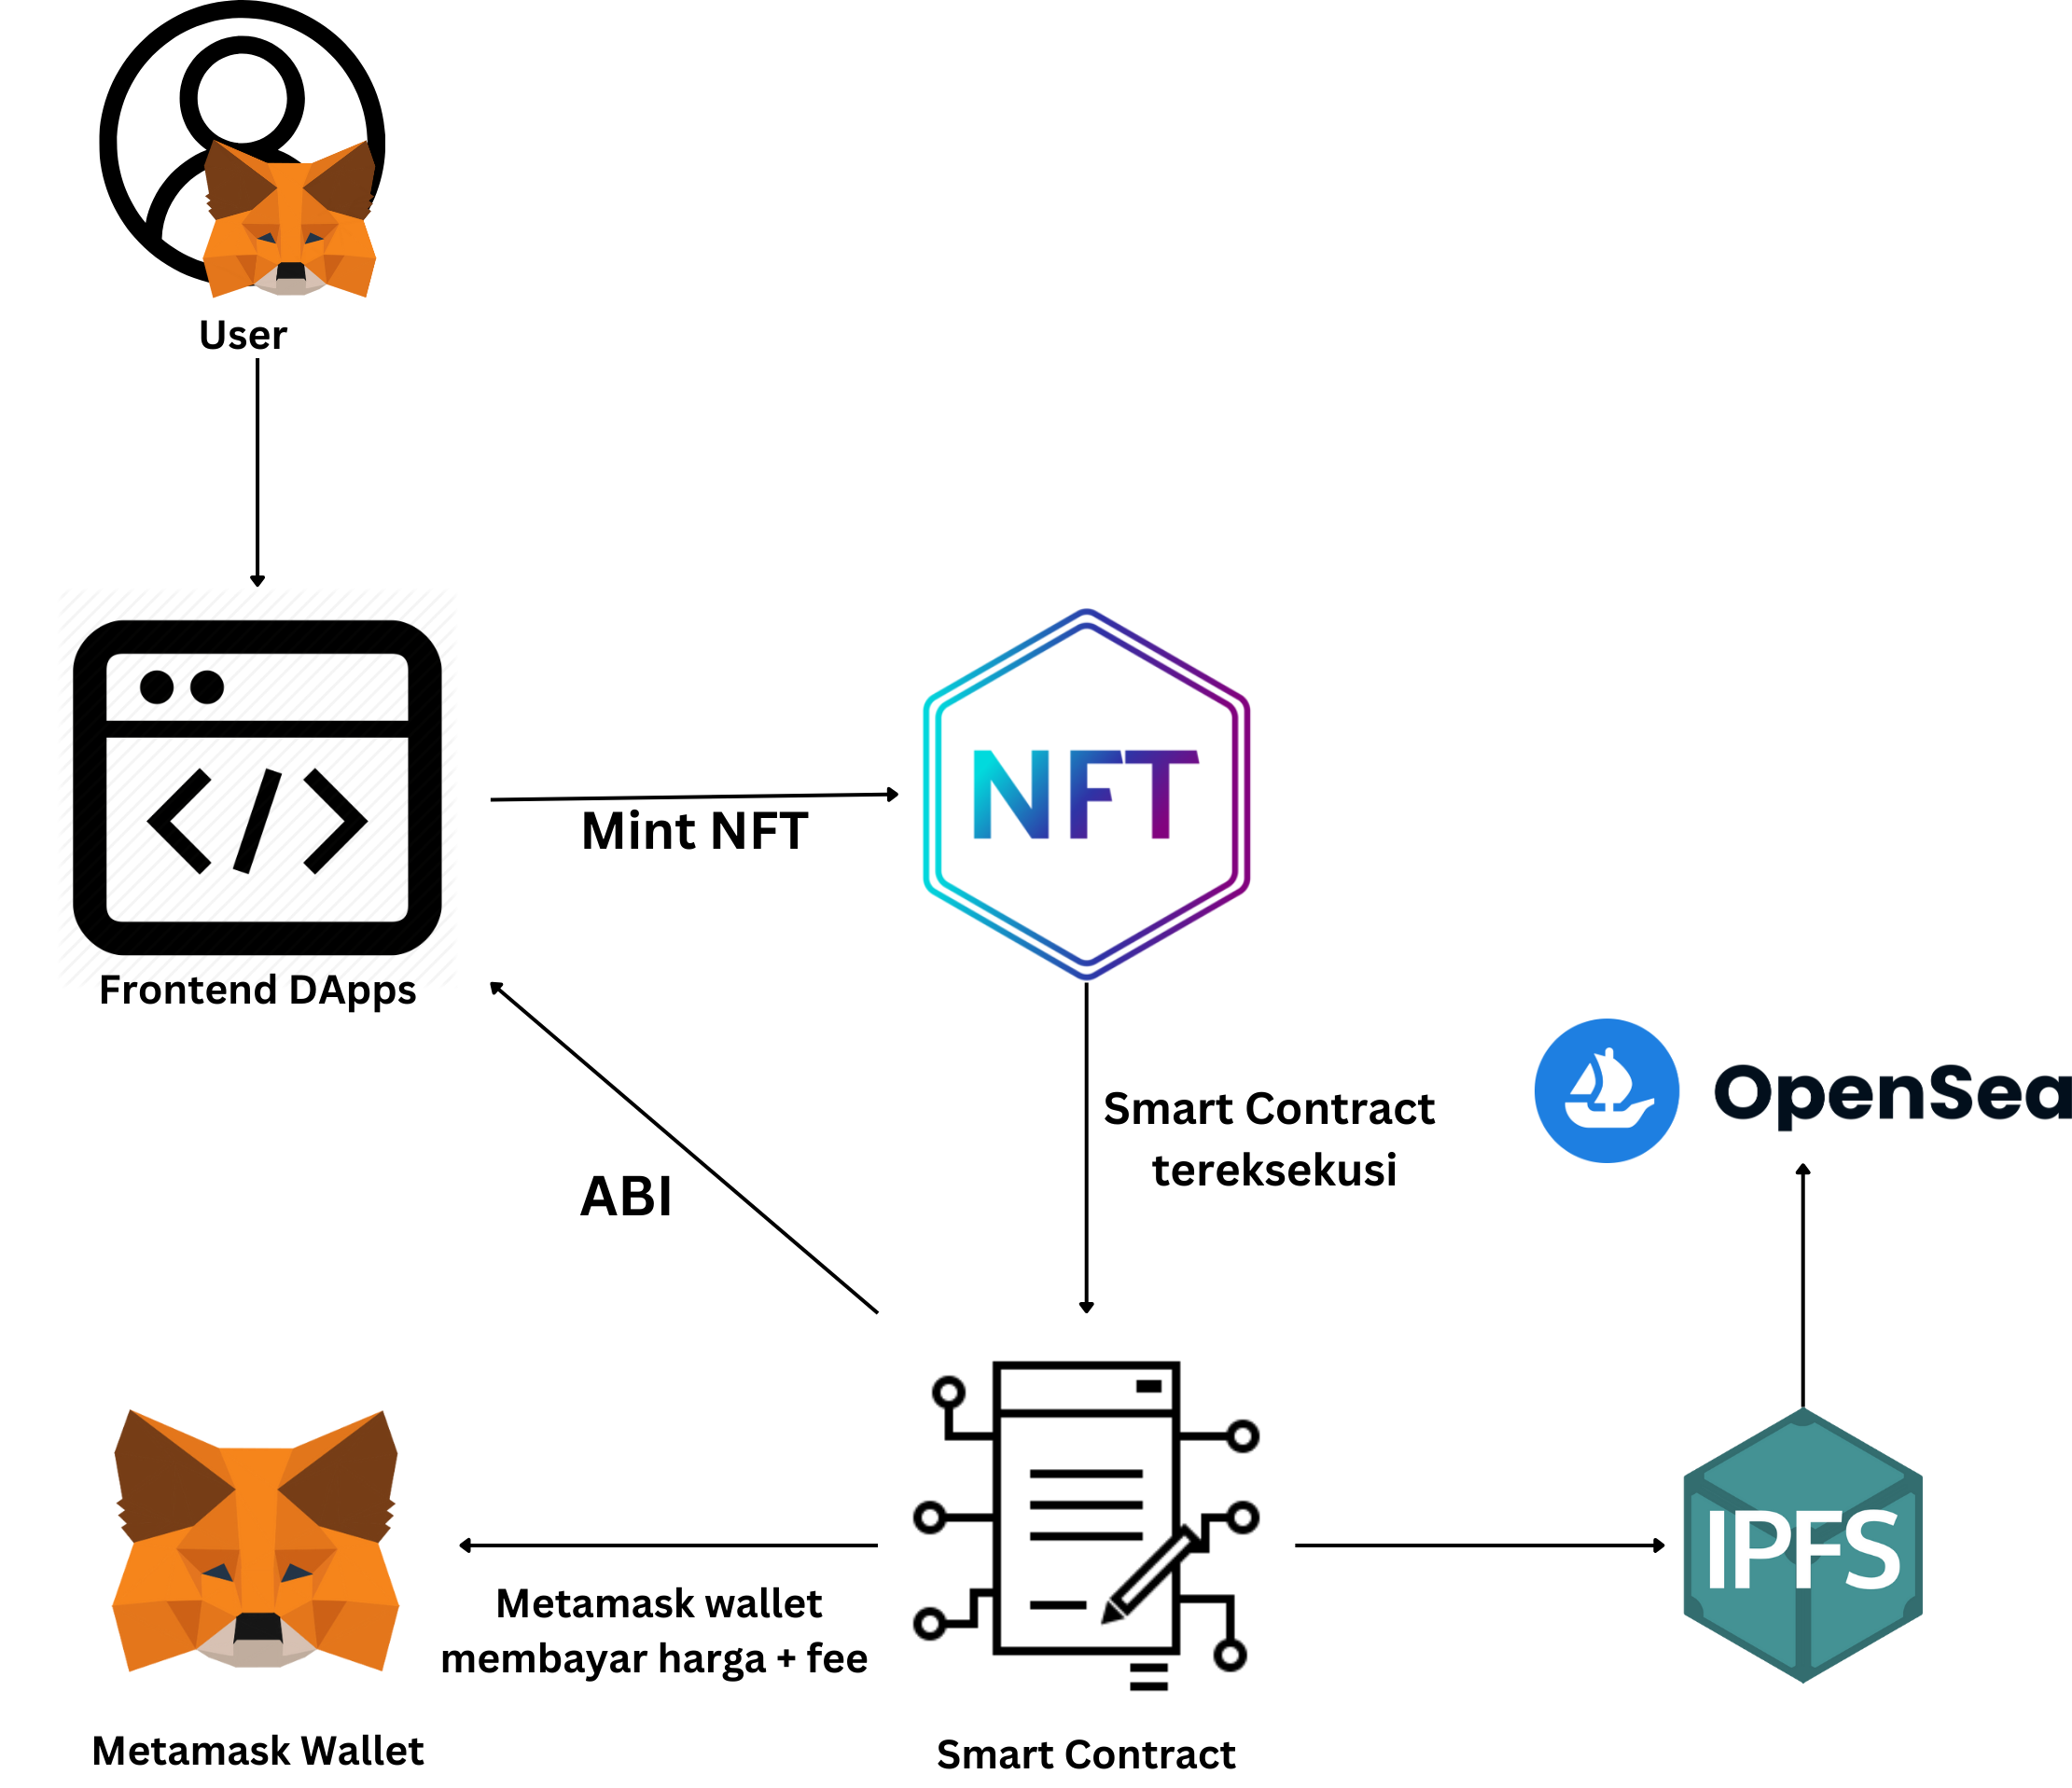
\includegraphics[scale=0.17]{gambar/desain_sistem_new.png}
  % Keterangan gambar yang diinputkan
  \caption{Arsitektur Sistem}
  % Label referensi dari gambar yang diinputkan
  \label{fig:flowtransaksi}
\end{figure}

Dalam pengembangan sistem \emph{smart contract} ini agar berjalan sesuai kehendak penulis untuk memenuhi tugas akhir ini, penulis membuat suatu arsitektur sistem. Pada arsitektur sistem ini, terdapat role \emph{user} yang dapat menjadi \emph{owner} dari suatu \emph{token} dan \emph{user} merupakan pihak yang memiliki akses terbatas terhadap suatu token dalam waktu yang telah ditentukan. Kemudian juga terdapat \emph{front end} untuk melakukan proses minting dari token NFT. Untuk dapat mengakses \emph{front end} baik owner ataupun user harus terhubung menggunakan wallet dari Metamask dalam berinteraksi.

Pada \emph{front end} akan terhubung dengan \emph{smart contract} ketika pengguna melakukan Minting dimana prosesnya pengguna mengunggah aset digital yang dimiliki dan diunggah ke IPFS melakukan aplikasi backend dan akan mengembalikan Content Identifier (CID). CID merupakan sebuah address file dalam IPFS yang digunakan untuk mengakses file tersebut. CID yang diperoleh kemudian akan diunggah ke jaringan \emph{blockchain} dan menjadi suatu token. Data-data mengenai NFT yang tersedia dapat langsung diperoleh \emph{frontend} melalui \emph{smart contract} pada \emph{blockchain}. 


\subsection{Flow Pembelian NFT}
\begin{figure} [H] \centering
  % Nama dari file gambar yang diinputkan
  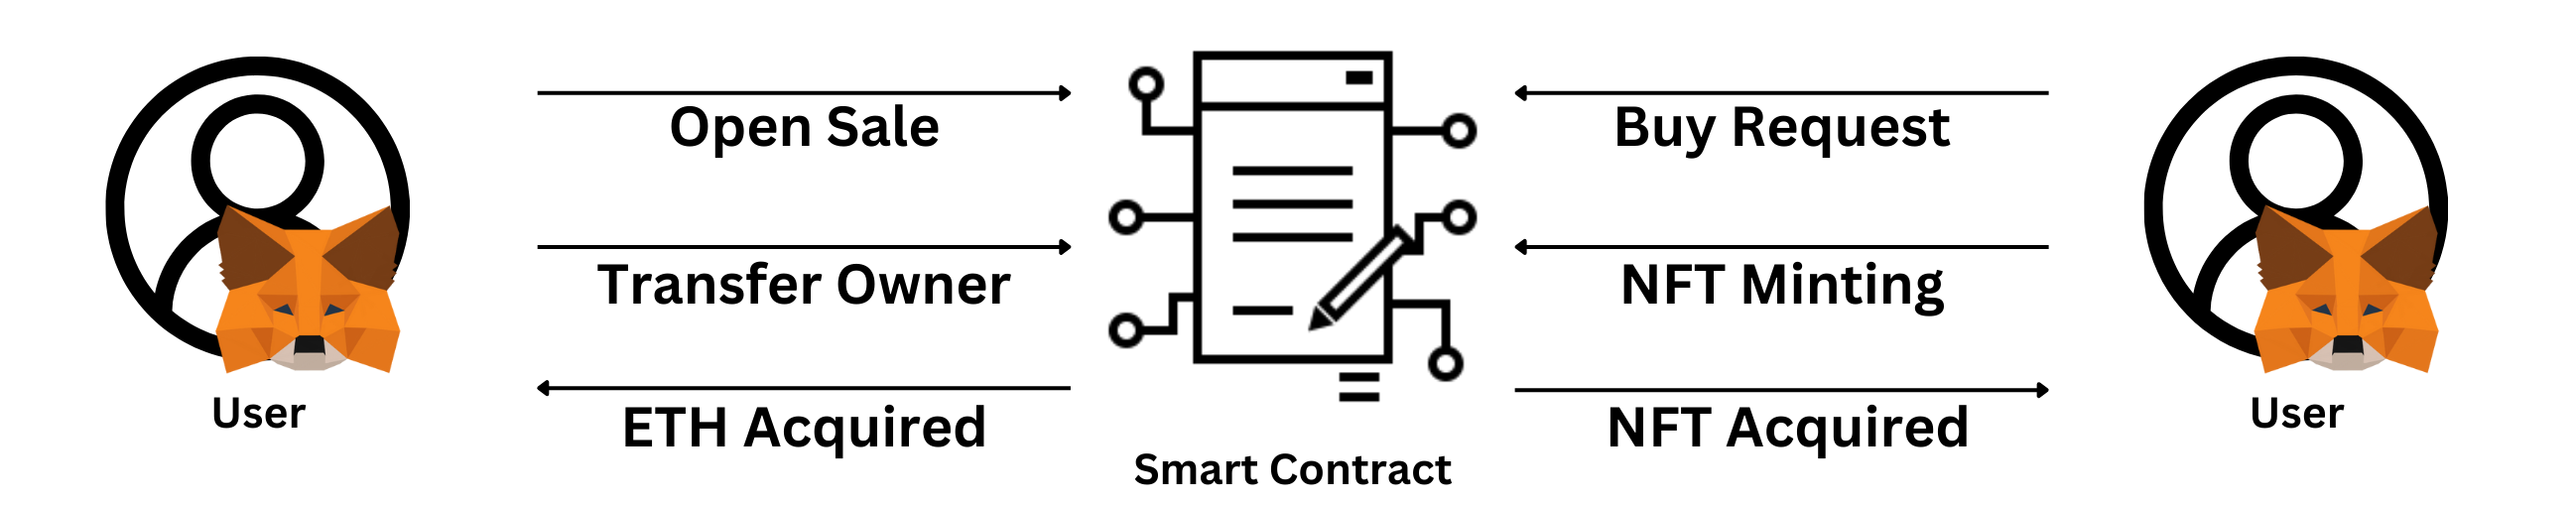
\includegraphics[scale=0.22]{gambar/flow_transaksi.png}
  % Keterangan gambar yang diinputkan
  \caption{Flow Pembelian NFT}
  % Label referensi dari gambar yang diinputkan
  \label{fig:flowtransaksi}
\end{figure}

Pada sistem ini terdapat juga fitur untuk melakukan pembelian NFT. Pembelian pada \emph{smart contract} yang akan dikembangkan menggunakan fungsi dari \emph{interface} token basis ERC-721. Interface ini memungkinkan token non-fungible diperjual belikan dalam satu kontrak. Kontrak ini akan tereksekusi ketika pengguna kedua (pembeli) melakukan pembelian token milik pengguna pertama (penjual). Kemudian pembeli melakukan minting NFT pada \emph{smart contract} dan juga penjual melakukan pemindahan kepemilikan dari NFT. Setelah proses itu selesai tereksekusi, pembeli mendapatkan NFT dan juga penjual mendapatkan mata uang kripto dari hasil penjualannya.

\subsection{Metadata}

\lstinputlisting[
  caption={Metadata pada NFT},
  label={lst:metadatanft}
]{program/A.json}

Dalam standar ERC-721, setiap NFT diwakili oleh metadata, yang merupakan kumpulan data mendetail mengenai konten Naturretnya dalam format JSON (JavaScript Object Notation). Metadata ini biasanya berisi informasi seperti nama, deskripsi, dan sebuah tautan ke gambar, yang semua dapat disesuaikan sesuai dengan kebutuhan aplikasi desentralisasi yang sedang dikembangkan. Struktur data ini disimpan dalam bentuk \emph{array} yang berisi objek-objek dalam format JSON, memungkinkan fleksibilitas tinggi dalam menyesuaikan data yang terkait dengan masing-masing NFT.

\subsection{Minting}
\begin{figure} [H] \centering
  % Nama dari file gambar yang diinputkan
  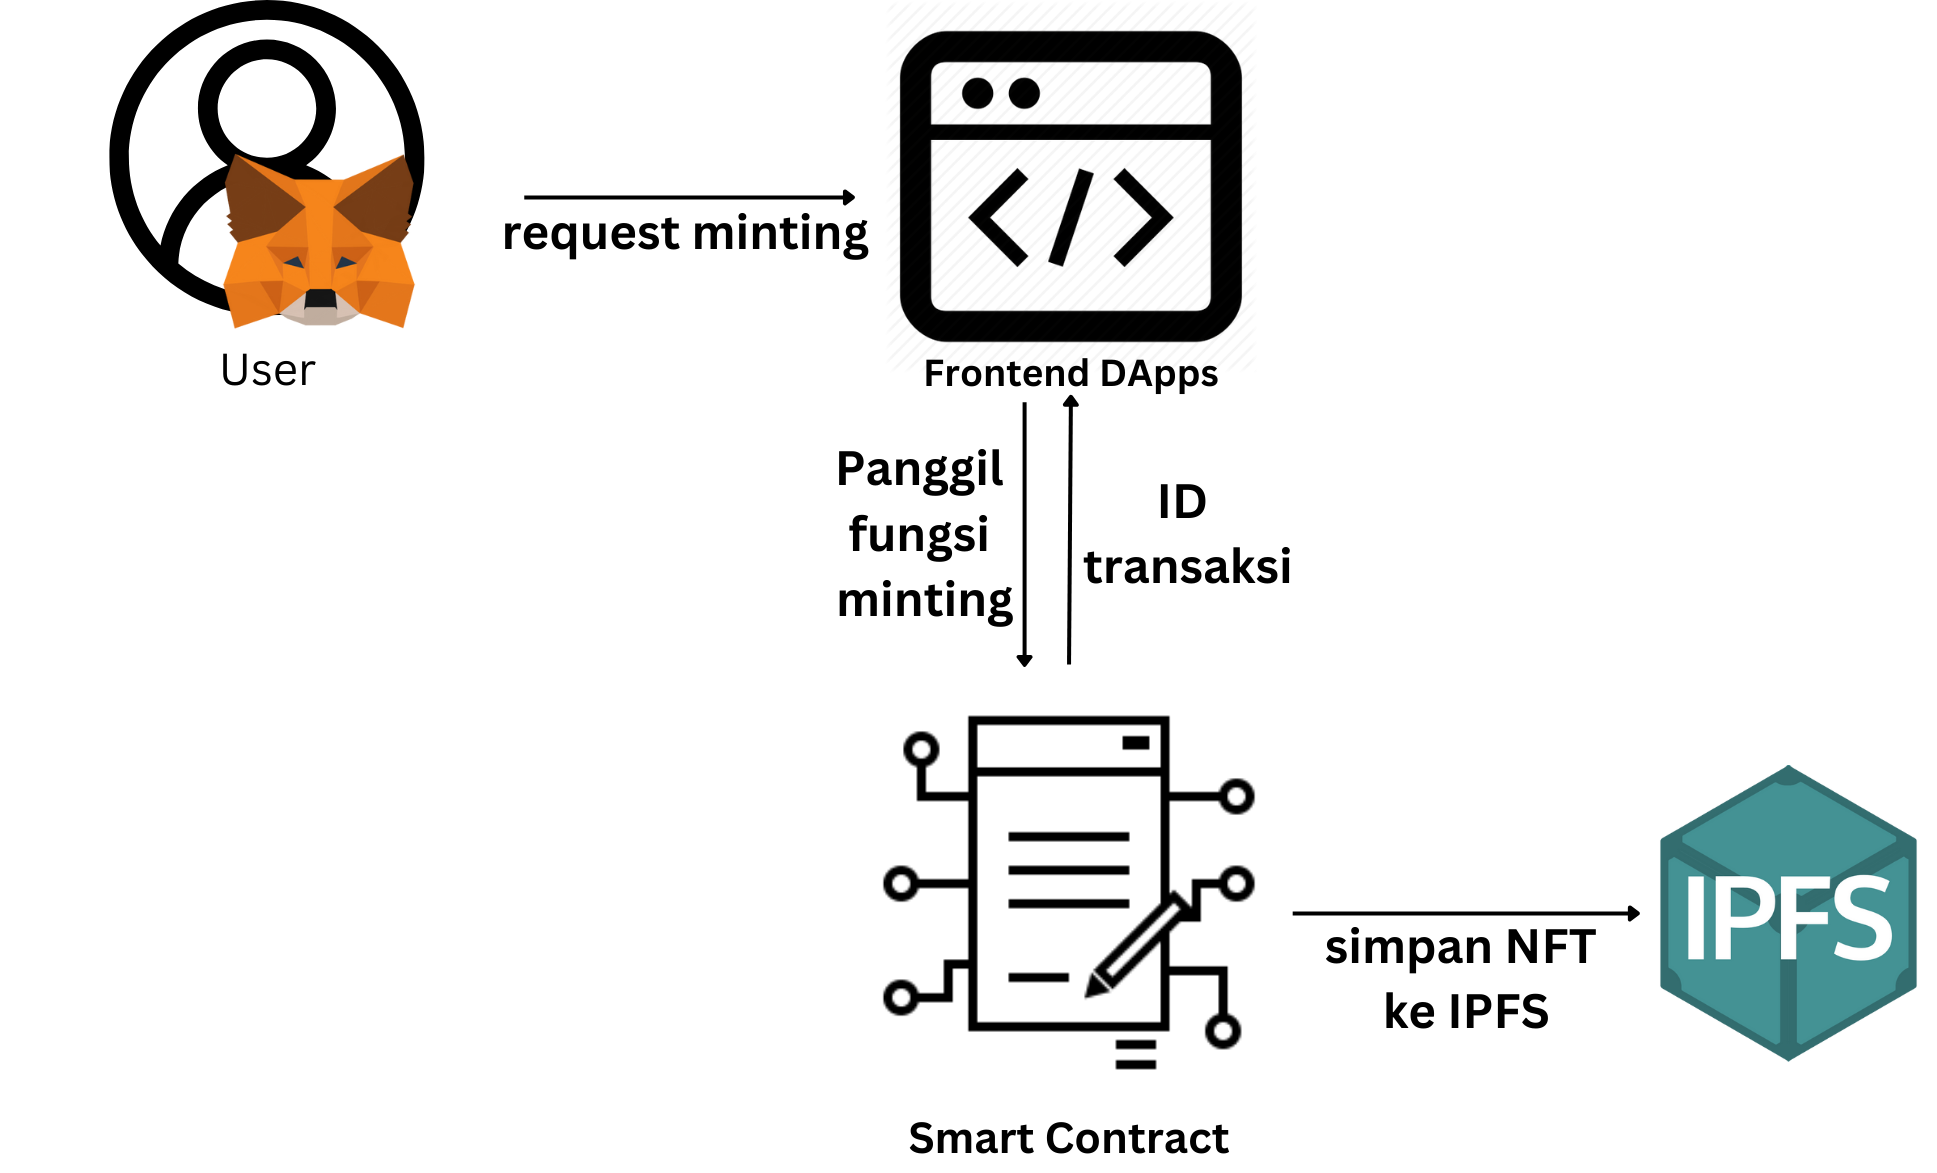
\includegraphics[scale=0.25]{gambar/proses_minting.png}
  % Keterangan gambar yang diinputkan
  \caption{Proses Minting}
  % Label referensi dari gambar yang diinputkan
  \label{fig:prosesminting}
\end{figure}


Proses \emph{minting} adalah langkah awal di mana sebuah NFT baru dibuat di dalam sebuah \emph{platform}. Selama proses ini, berbagai informasi penting tentang NFT tersebut harus ditentukan, termasuk nama, deskripsi, kategori, jumlah suplai yang tersedia, dan aset visual yang mewakili NFT, yang bisa berupa gambar 2D, model 3D, atau video. Harga awal, koleksi yang termasuk NFT, serta atribut lainnya juga perlu ditetapkan. Setelah proses minting selesai, data dari NFT yang baru dibuat ini akan disimpan dalam InterPlanetary File System (IPFS), yang memungkinkan penyimpanan dan akses data yang terdesentralisasi. Penyimpanan ini memastikan bahwa semua informasi terkait, seperti kepemilikan yang tercatat dalam atribut NFT, dapat diakses secara permanen dan aman.

\vspace{0.5 cm}

\section{Tools yang digunakan}
\label{sec:tools}
\subsection{Solidity}

Solidity adalah bahasa pemrograman tingkat tinggi yang dirancang khusus untuk menulis \emph{smart contracts} di dalam platform \emph{blockchain} Ethereum. Bahasa pemrograman ini dirancang khusus untuk mengatasi \emph{smart contracts}, menyediakan sintaks yang mendukung variabel, fungsi, serta pernyataan kontrol yang diperlukan untuk kontrak yang andal. Solidity juga menyertakan fitur-fitur keamanan yang dapat membantu pengembang menghindari kerentanannya seperti serangan \emph{reentrancy} dan \emph{overflows}. Solidity dirancang untuk berjalan di atas Ethereum Virtual Machine (EVM), yang merupakan lingkungan komputasi Ethereum.

\subsection{Metamask}

Metamask adalah perangkat lunak yang memungkinkan pengguna untuk mengelola kripto-currency, terutama Ether (ETH), serta berinteraksi dengan aplikasi dan layanan terdesentralisasi di \emph{blockchain} Ethereum. Metamask hadir sebagai sebuah Extension pada Browser. 

\subsection{Hardhat}

Hardhat adalah framework pengembangan \emph{smart contracts} yang didesain khusus untuk mempermudah pengembangan, pengujian, dan distribusi \emph{smart contracts}, Hardhat menyediakan berbagai alat dan fungsi yang kuat bagi pengembang blockchain.

\subsection{Ganache}

Ganache adalah alat simulasi \emph{blockchain} Ethereum yang digunakan secara luas dalam pengembangan dan pengujian \emph{smart contracts} dan aplikasi berbasis Ethereum. Ini memungkinkan pengembang untuk membuat jaringan \emph{blockchain} lokal yang dapat dijalankan di komputer mereka sendiri, mirip dengan jaringan Ethereum nyata, tetapi tanpa memerlukan sumber daya yang besar atau biaya transaksi yang sebenarnya.

\subsection{InterPlanetary File System}
InterPlanetary File System (IPFS) adalah protokol \emph{hypermedia} terdistribusi yang bertujuan untuk membuat web lebih cepat, aman, dan terbuka. IPFS telah menjadi populer di kalangan pengembang, terutama dalam pengembangan \emph{smart contract} untuk Non-Fungible Tokens (NFTs). Pada dasarnya, IPFS memungkinkan penyimpanan dan berbagi data dalam jaringan terdistribusi yang mirip dengan sistem peer-to-peer. Setiap file dan semua blok dalamnya diberi \emph{hash kriptografis} yang unik, yang bertindak sebagai alamat unik di jaringan.

Dalam konteks NFT, IPFS sangat berguna karena menyediakan solusi untuk tidak tergantung pada server tunggal atau lokasi penyimpanan yang bisa menjadi titik kegagalan. Misalnya, jika \emph{metadata} atau aset digital NFT seperti gambar, video, atau file audio disimpan hanya di server terpusat, ada risiko bahwa data tersebut bisa hilang atau dihapus. Menggunakan IPFS, file tersebut disimpan di beberapa node dalam jaringan, meningkatkan ketahanan dan ketersediaan data. Setiap kali file diminta, IPFS mengambil beberapa potongan dari banyak node, bukan mengambil seluruh file dari satu lokasi, mempercepat waktu pemuatan dan mengurangi beban pada jaringan.

\subsection{React.js}
React.js adalah sebuah pustaka JavaScript yang populer dan kuat untuk membangun antarmuka pengguna, atau lebih dikenal dengan istilah UI (\emph{User Interface}). Keunggulan React.js terletak pada kemampuannya untuk membangun aplikasi web yang dinamis dengan cara yang efisien dan mudah. React.js memungkinkan pengembang untuk membuat komponen UI yang besar dan kompleks, yang dapat dikelola dengan baik melalui penggunaan state dan props yang memberikan cara untuk \emph{data flow} dan \emph{re-rendering} yang efisien. 

Menggunakan React.js, pengembang dapat memanfaatkan library seperti Web3.js atau Ethers.js untuk berinteraksi langsung dengan \emph{blockchain Ethereum}, tempat \emph{smart contract} di-\emph{deploy}. Hal ini memungkinkan aplikasi untuk melakukan \emph{query} dan memperbarui \emph{blockchain} dengan transparan, menampilkan informasi seperti kepemilikan NFT, sejarah transaksi, dan \emph{metadata} NFT secara \emph{real-time}. 

\subsection{Web3.js}
Web3.js adalah sebuah pustaka JavaScript yang sangat penting untuk pengembangan aplikasi web yang berinteraksi dengan \emph{blockchain} Ethereum, khususnya dalam ekosistem Web 3.0. Library ini memungkinkan pengembang \emph{frontend} untuk berkomunikasi langsung dengan \emph{node} Ethereum, memanfaatkan fungsionalitas \emph{blockchain} seperti \emph{smart contracts}, transaksi, dan manajemen akun langsung dari browser pengguna.

Integrasi Web3.js dalam aplikasi React.js memungkinkan pengembang untuk memanfaatkan \emph{hook} dan komponen React untuk merespons perubahan \emph{state} pada \emph{blockchain} secara \emph{real-time}. Ini termasuk pembaruan saldo, perubahan status transaksi, dan pembaruan pada data \emph{smart contract}. Fungsi ini memperkuat pengalaman pengguna dengan memberikan tampilan yang konsisten dan \emph{up-to-date} dari status \emph{blockchain}, yang sangat penting dalam aplikasi yang menuntut keandalan dan transparansi tinggi.

\subsection{Ethers.js}
Ethers.js adalah sebuah \emph{library} JavaScript ringan yang dirancang untuk berinteraksi dengan Ethereum \emph{blockchain}. \emph{Library} ini sangat cocok untuk digunakan dalam pengembangan aplikasi \emph{frontend} dengan React.js karena menawarkan API yang sederhana dan modular, memudahkan pengembangan aplikasi desentralisasi (DApps) yang efisien. Ethers.js menyediakan fungsi-fungsi penting seperti penyambungan dengan \emph{wallet} pengguna, pembuatan dan pengiriman transaksi, serta interaksi dengan \emph{smart contract}.

Dalam pengembangan dengan React.js, Ethers.js membantu mengintegrasikan fungsi \emph{blockchain} ke dalam komponen React dengan cara yang bersih dan efektif. Misalnya, dengan menggunakan React \emph{hooks} seperti \emph{useState} dan \emph{useEffect}, pengembang dapat dengan mudah mengintegrasikan status dari \emph{Ethereum blockchain} ke dalam UI aplikasi, memperbarui UI secara \emph{real-time} ketika ada perubahan pada \emph{blockchain} seperti konfirmasi transaksi atau perubahan pada data \emph{contract}.



\section{Metode Yang Digunakan}

% Contoh input gambar dengan format *.jpg
\begin{figure} [H] \centering
  % Nama dari file gambar yang diinputkan
  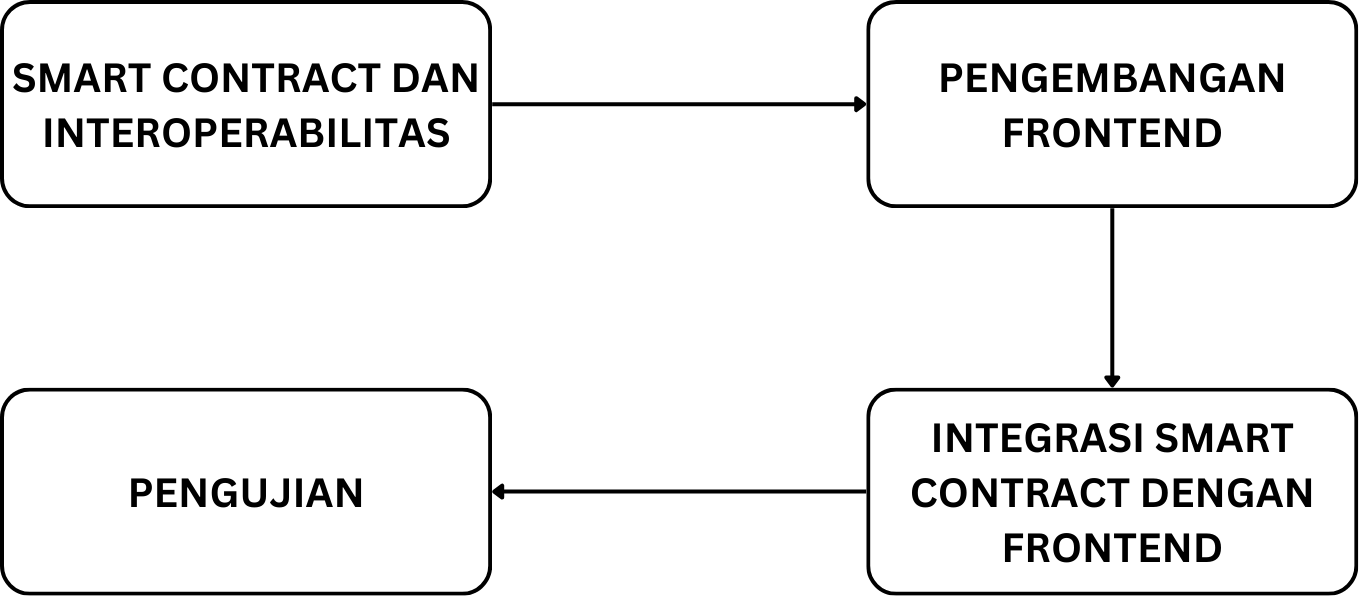
\includegraphics[scale=0.25]{gambar/metodologi_new.png}
  % Keterangan gambar yang diinputkan
  \caption{Metodologi Penelitian Yang Digunakan}
  % Label referensi dari gambar yang diinputkan
  \label{fig:flowtransaksi}
\end{figure}

\subsection{Smart Contract dan Interoperabilitas}
Pada tahapan ini, penulis mengembangkan sistem \emph{smart contract} yang digunakan untuk pembuatan token yang berinteroperabilitas menggunakan bahasa pemrograman Solidity. Sistem \emph{smart contract} ini digunakan sebagai jembatan untuk memperoses request dari yang dihasilkan dari interaksi pengguna pada \emph{frontend} ke jaringan \emph{blockchain}. Pada \emph{smart contract} yang telah di-\emph{compile} akan muncul ABI (\emph{Application Binary Interface}) yang dapat digunakan pada \emph{frontend} sebagai encoding dan decoding data yang memungkinkan \emph{frontend} aplikasi untuk mengirim instruksi yang tepat ke \emph{smart contract} dan memahami data yang dikembalikan olehnya. Dalam \emph{smart contract} yang dibuat oleh penulis terdapat beberapa fungsi yang dibuat sebagai inti pada token yang dikembangkan.

\subsubsection{Fungsi Mint}
Fungsi Mint dalam konteks \emph{smart contract } ERC-721 yang digunakan untuk \emph{minting} token NFT merupakan komponen krusial dalam mengelola penerbitan token baru. Ini diakses secara publik dan dapat menerima Ether, yang memungkinkan pembayaran langsung selama proses \emph{minting}.

\begin{lstlisting}[caption=Fungsi Mint]
FUNSI mint(_tokenURI: STRING) MENGEMBALIKAN BILANGAN BULAT:
    TAMBAHKAN tokenCount SEBANYAK 1
    JALANKAN _safeMint DENGAN PARAMETER (msg.sender, tokenCount)
    JALANKAN _setTokenURI DENGAN PARAMETER (tokenCount, _tokenURI)
    KEMBALIKAN tokenCount
AKHIR FUNGSI
\end{lstlisting}

\begin{itemize}
    \item \emph{Increment tokenCount}
    
    Pada awalnya, fungsi ini meningkatkan variabel \emph{tokenCount}. Variabel ini bertindak sebagai pengidentifikasi unik untuk setiap token baru; ini memastikan bahwa setiap token yang dicetak memiliki ID yang unik.

    \item \emph{Mint Token}
    
    Selanjutnya, fungsi memanggil metode \emph{\texttt{\_safeMint}}. Metode ini bertanggung jawab atas penciptaan token sebenarnya. Ini menetapkan kepemilikan token yang baru dicetak kepada pemanggil fungsi (\emph{msg.sender}), yang biasanya adalah pengguna yang berinteraksi dengan kontrak. Penggunaan \emph{\texttt{\_safeMint}} (dibandingkan \emph{\texttt{\_mint}}) memastikan pemeriksaan tambahan ada untuk mencegah token dikirim ke kontrak yang tidak siap untuk menanganinya, yang dapat mencegah kehilangan token secara tidak sengaja.

    \item \emph{Set Token URI}
    
    Setelah mencetak token, fungsi memperbarui metadata token dengan memanggil \emph{\texttt{\_tokenURI}}. Metode ini mengaitkan URI yang disediakan (\emph{\texttt{\_tokenURI}}) dengan ID token. URI biasanya mengarah ke file JSON yang di-\emph{host} secara eksternal yang berisi \emph{metadata} tentang token, seperti nama, deskripsi, dan URL gambar. Metadata ini memperkaya token dan dapat digunakan untuk memberikan informasi lebih rinci tentang aset digital.

    \item \emph{Return tokenCount}
    
    Terakhir, fungsi mengembalikan \emph{tokenCount}, yang merupakan pengidentifikasi unik dari token yang baru dicetak. ID ini dapat digunakan oleh aplikasi eksternal atau fungsi kontrak lain untuk merujuk token spesifik ini.
\end{itemize}

Secara keseluruhan, fungsi \emph{mint} ini sangat penting untuk menciptakan aset digital baru di \emph{blockchain}, memberikan pengguna kemampuan untuk menghasilkan NFT unik yang dapat mewakili segala sesuatu mulai dari seni digital hingga \emph{real estate virtual}, memastikan setiap aset dapat diidentifikasi secara jelas melalui ID token yang unik.
    
\subsubsection{Fungsi \emph{lockToken}}
\begin{lstlisting}[caption=Fungsi lockToken]
FUNGSI lockToken(tokenId: BILANGAN BULAT):
    PASTIKAN _exists(tokenId) = TRUE dengan pesan "Token does not exist."
    ATUR _locked[tokenId] = TRUE
    KIRIMKAN EVENT TokenLocked dengan (tokenId, msg.sender)
AKHIR FUNGSI
\end{lstlisting}

\begin{itemize}
    \item Pemeriksaan Keberadaan Token
    
    Fungsi ini memulai dengan memeriksa apakah token dengan ID yang diberikan benar-benar ada. Ini dilakukan melalui pemanggilan fungsi \emph{\texttt{\_exists}} yang memeriksa dalam basis data smart contract apakah token tersebut sudah dicetak dan masih ada. Jika token tidak ditemukan, fungsi akan memberikan error dan berhenti, dengan pesan "Token does not exist."

    \item Mengunci Token
    
    Jika token ditemukan, fungsi kemudian melanjutkan untuk mengunci token tersebut dengan mengatur nilai dari mapping \emph{\texttt{\_locked}} untuk tokenId yang bersangkutan menjadi true. Ini efektif membatasi fungsi smart contract yang dapat berinteraksi dengan token tersebut, khususnya mencegah transfer atau transaksi lain yang mungkin mengubah kepemilikan atau status token.

    \item Emit Event
    
    Setelah token berhasil dikunci, fungsi kemudian memicu event TokenLocked yang menandakan bahwa token telah dikunci. Event ini mencatat tokenId dan alamat yang memicu fungsi (biasanya pemilik atau pengontrol kontrak, sebagaimana ditandai oleh modifier onlyOwner). Event ini bisa digunakan untuk memberitahukan pengguna atau aplikasi lain yang berinteraksi dengan blockchain bahwa token tersebut sekarang berada dalam status terkunci dan tidak dapat dioperasikan atau dipindahkan hingga dibuka kunci.
\end{itemize}

Secara keseluruhan, fungsi \emph{lockToken} berperan penting dalam menjamin keamanan dan integritas transaksi yang melibatkan NFT, khususnya dalam skenario yang melibatkan operasi lintas rantai atau ketika sebuah token sedang menunggu konfirmasi transaksi yang kritis. Fungsi ini membantu memastikan bahwa tidak ada pihak yang tidak berwenang atau proses otomatis lainnya yang dapat mengganggu proses hukum atau komersial yang sedang berlangsung.

\subsubsection{Fungsi \emph{unlockToken}}
Fungsi unlockToken dalam \emph{smart contract} bertujuan untuk membuka kunci token yang sebelumnya telah dikunci. Fungsi ini sangat penting dalam manajemen aset dalam \emph{smart contract}, terutama dalam kasus penggunaan seperti transaksi lintas rantai atau ketika token harus dikunci untuk alasan keamanan atau administratif.

\begin{lstlisting}[caption=Fungsi unlockToken]
FUNGSI unlockToken(tokenId: BILANGAN BULAT)
    PASTIKAN _locked[tokenId] = TRUE dengan pesan "Token is not locked."
    ATUR _locked[tokenId] = FALSE
    KIRIMKAN EVENT TokenUnlocked dengan (tokenId, msg.sender)
AKHIR FUNGSI
\end{lstlisting}

\begin{itemize}
    \item Verifikasi Status Kunci
    
    Langkah pertama dalam fungsi ini adalah memastikan bahwa token yang ditentukan benar-benar dalam keadaan terkunci. Ini dilakukan dengan memeriksa mapping \emph{\texttt{\_locked}} untuk tokenId yang diberikan. Jika nilai dari mapping ini adalah false, yang berarti token tidak terkunci, maka fungsi akan menghasilkan error dan menghentikan eksekusi lebih lanjut dengan pesan "Token is not locked." Ini mencegah upaya untuk membuka kunci token yang tidak perlu atau yang mungkin telah secara tidak sengaja terbuka.

    \item Membuka Kunci Token
    
    Jika token memang terkunci, fungsi kemudian mengatur nilai dalam mapping \emph{\texttt{\_locked}} untuk tokenId tersebut menjadi false, secara efektif membuka kunci token tersebut. Ini mengizinkan token untuk berpartisipasi dalam transaksi dan interaksi lainnya sesuai dengan aturan smart contract lainnya.

    \item Emit Event
    
    Setelah token berhasil dibuka kunci, fungsi memicu event TokenUnlocked yang menandakan bahwa token tersebut telah dibuka kunci. Event ini mencatat tokenId dan alamat pengguna yang menjalankan fungsi (dijamin adalah pemilik atau pengontrol kontrak melalui penggunaan modifier onlyOwner). Event ini berguna untuk audit, pemantauan keamanan, dan sebagai bukti dalam aplikasi yang berinteraksi dengan smart contract bahwa token telah kembali ke status normal dan siap untuk dipindahkan atau digunakan.
\end{itemize}

Secara keseluruhan, fungsi unlockToken memainkan peran krusial dalam memastikan fleksibilitas dan keamanan dalam pengelolaan NFT dan aset digital lainnya. Fungsi ini memungkinkan pemilik atau pengontrol kontrak untuk secara efektif mengelola akses dan kontrol atas aset digital, memastikan bahwa aset tersebut hanya terkunci ketika benar-benar diperlukan dan bisa dibuka kembali ketika kondisi memungkinkan.

\subsubsection{Fungsi \emph{bridgeTransfer}}
Fungsi \emph{bridgeTransfer} dirancang untuk memungkinkan pemindahan token yang aman antara berbagai blockchain atau sub-jaringan, sebuah proses yang sering disebut sebagai "\emph{bridging}". Fungsi ini memastikan bahwa NFT (Non-Fungible Token) hanya dapat ditransfer setelah memenuhi kriteria keamanan tertentu.

\begin{lstlisting}[caption=Fungsi bridgeTransfer]
FUNGSI bridgeTransfer(_to: ALAMAT, _tokenId: BILANGAN BULAT)
    PASTIKAN _locked[_tokenId] = TRUE dengan pesan "Token must be locked before bridging"
    TRANSFER_TOKEN dari owner() ke _to dengan _tokenId
    KIRIMKAN EVENT TokenBridged dengan (_tokenId, owner(), _to)
AKHIR FUNGSI
\end{lstlisting}

\begin{itemize}
    \item Verifikasi Kondisi Kunci
    
    Langkah awal dalam fungsi ini adalah memastikan bahwa token yang ingin ditransfer sudah terkunci. Ini dilakukan dengan memeriksa nilai dari mapping \emph{\texttt{\_locked}} untuk tokenId yang diberikan. Jika token ini tidak terkunci, fungsi akan mengeluarkan kesalahan dan menghentikan proses lebih lanjut dengan pesan "\emph{Token must be locked before bridging}". Kondisi ini memastikan bahwa token hanya dipindahkan setelah melalui tahapan penguncian yang mencegah penggunaan atau transfer yang tidak sah sebelumnya.

    \item Eksekusi Transfer
    
    Setelah dipastikan bahwa token terkunci, fungsi selanjutnya melakukan transfer NFT dari pemilik saat ini ke alamat tujuan yang ditentukan (\emph{\texttt{\_to}}). Transfer ini dilakukan menggunakan fungsi \emph{\texttt{\_transfer}} yang merupakan bagian dari standar \emph{ERC-721}, memungkinkan perubahan kepemilikan NFT dalam \emph{blockchain}.

    \item Pencatatan Event
    
    Setelah transfer berhasil, fungsi mengirim event \emph{TokenBridged}. Event ini mencatat tokenId, alamat pemilik sebelum transfer (\emph{owner())}), dan alamat tujuan (\emph{\texttt{\_to}}). Event ini penting untuk audit dan pemantauan, memungkinkan aplikasi dan layanan yang terhubung untuk merespons atau mengakui transfer NFT lintas rantai.
\end{itemize}

Dengan cara ini, \emph{bridgeTransfer} menyediakan mekanisme yang efisien dan aman untuk mengintegrasikan fungsi interoperabilitas dalam \emph{smart contract} NFT, memungkinkan aset digital untuk berpindah antar ekosistem \emph{blockchain} sambil mempertahankan tingkat keamanan dan verifikasi yang ketat. Fungsi ini sangat penting dalam ekosistem \emph{blockchain} yang semakin terhubung, di mana NFT dan aset digital lainnya sering perlu beroperasi di berbagai platform dan jaringan.

\subsection{Pengembangan Frontend}
Pada tahap pengembangan frontend dalam proyek ini, kami memilih React.js sebagai kerangka kerja utama karena fleksibilitas dan efisiensinya dalam membangun antarmuka pengguna yang dinamis dan responsif. React.js memungkinkan pembuatan komponen yang dapat digunakan kembali, yang sangat meningkatkan efisiensi pengembangan dengan memungkinkan kami untuk membangun UI yang kompleks dari komponen yang lebih kecil dan termodularisasi.

Untuk mengintegrasikan aplikasi React dengan blockchain Ethereum, kami menggunakan dua pustaka utama: ethers.js dan web3.js. Kedua pustaka ini menyediakan fungsionalitas yang diperlukan untuk berinteraksi dengan Ethereum blockchain, tetapi dengan pendekatan yang sedikit berbeda. Ethers.js dikenal dengan API-nya yang minimalis dan mudah digunakan, yang sangat cocok untuk proyek-proyek dengan kebutuhan yang lebih sederhana dan lebih fokus pada pembacaan serta penulisan data ke blockchain. Pustaka ini menyediakan fungsi yang kuat untuk berinteraksi dengan smart contracts, seperti mengirim transaksi, membaca status kontrak, dan menangani notifikasi event.

Di sisi lain, web3.js adalah pustaka yang lebih luas yang sering digunakan untuk proyek yang memerlukan integrasi yang lebih kompleks dengan Ethereum. Web3.js menyediakan modul yang lebih komprehensif dan mendukung interaksi yang lebih beragam dengan blockchain, termasuk pengelolaan akun, komputasi gas, dan langganan event yang lebih canggih. Kedua pustaka ini, ketika digunakan bersama-sama atau secara terpisah, memberikan fleksibilitas yang sangat dibutuhkan dalam pengembangan frontend untuk aplikasi berbasis blockchain.

\subsection{Integrasi Smart Contract dengan Frontend}
Pada tahap ini memungkinkan aplikasi yang dibangun dengan React.js untuk berinteraksi secara langsung dengan smart contract yang telah dideploy di jaringan Ethereum. Untuk mencapai integrasi ini, kami menggunakan pustaka ethers.js, yang menyediakan antarmuka yang bersih dan mudah digunakan untuk berkomunikasi dengan Ethereum.

Setelah smart contract dikembangkan dan dideploy, ABI (Application Binary Interface) dari contract tersebut digunakan untuk membangun sebuah instance contract dalam aplikasi React. ABI memungkinkan frontend untuk mengetahui fungsi-fungsi apa saja yang tersedia dalam smart contract, termasuk variabel dan tipe data yang digunakan. Dengan informasi ini, ethers.js dapat memanggil fungsi-fungsi tersebut seperti fungsi safeMint atau transferOwnership, sesuai dengan logika yang didefinisikan dalam contract.

Dalam aplikasi, kami mengonfigurasi ethers.js untuk terhubung dengan provider Ethereum, yang bisa berupa MetaMask atau node Ethereum lainnya. Ini memungkinkan aplikasi untuk mengirim transaksi dan memantau event yang diterbitkan oleh smart contract. Setiap kali pengguna berinteraksi dengan UI, seperti mengklik tombol untuk memint NFT atau mentransfer kepemilikan, permintaan tersebut diterjemahkan oleh ethers.js menjadi transaksi blockchain yang sesuai.

Selain itu, untuk meningkatkan keamanan dan keandalan aplikasi, kami juga mengimplementasikan penanganan error yang robust untuk mengatasi masalah yang mungkin terjadi selama interaksi dengan blockchain, seperti kegagalan transaksi atau masalah konektivitas. Dengan demikian, pengguna dapat menerima feedback yang tepat waktu dan akurat jika ada masalah yang terjadi selama proses transaksi.

\subsection{Pengujian}
Pada tahap ini terdapat beberapa langkah pengujian \emph{smart contract} yaitu pengujian unit dan juga pengujian integrasi.

\begin{itemize}
    \item Pengujian Unit
    Pada pengujian ini adalah fokus dalam memvalidasi setiap komponen secara individual. Dalam konteks frontend React.js, ini berarti menguji komponen-komponen secara terpisah untuk memastikan bahwa mereka berperilaku sesuai dengan ekspektasi. Pengujian unit juga dilakukan pada fungsi-fungsi smart contract untuk memverifikasi logika bisnisnya, seperti fungsi minting atau transfer token. Pengujian ini biasanya dilakukan dengan bantuan framework React untuk frontend dan  Hardhat untuk smart contracts.

    \item Pengujian Integrasi
    Setelah pengujian unit, langkah berikutnya adalah pengujian integrasi, yang memastikan bahwa semua komponen dalam aplikasi bekerja dengan baik saat digabungkan. Dalam konteks integrasi smart contract, ini melibatkan menguji interaksi antara frontend React.js dan smart contract melalui ethers.js atau web3.js. Pengujian integrasi membantu mendeteksi masalah pada alur data antara frontend dan blockchain, termasuk validasi transaksi dan pembaruan state yang benar.
\end{itemize}
